\documentclass{article}
%\documentstyle[11pt,handout,psfig]{article}

\usepackage{fullpage,amssymb,amsmath,tikz,forest,float,subcaption,braket}
\usetikzlibrary{arrows.meta}
\usepackage{graphicx}
\usepackage{hyperref}
\hypersetup{
    colorlinks=true,
    linkcolor=blue,
    filecolor=magenta,      
    urlcolor=cyan,
}

\forestset{
    default preamble={
        for tree={
        	   font=\tiny,
            base=bottom,
            child anchor=north,
            align=center,
            s sep+=1.3cm,
    straight edge/.style={
        edge path={\noexpand\path[\forestoption{edge},thick,-{Latex}] 
        (!u.parent anchor) -- (.child anchor);}
    },
    if n children={0}
        {tier=word, draw, thick, rectangle}
        {
        		if n children={1}
        		{draw, thick, rectangle, parent anchor=south}
        		{draw, diamond, thick, aspect=2}
        },
    if n=1{%
    		if n'=1
    			{edge path={\noexpand\path[\forestoption{edge},thick,-{Latex}] 
        			(!u.parent anchor) -| (.child anchor);}}
        		{edge path={\noexpand\path[\forestoption{edge},thick,-{Latex}] 
        			(!u.parent anchor) -| (.child anchor) node[pos=.2, above] {Y};}}
        }{
        edge path={\noexpand\path[\forestoption{edge},thick,-{Latex}] 
        (!u.parent anchor) -| (.child anchor) node[pos=.2, above] {N};}
        }
        }
    }
}
\usepackage{xcolor}
\usepackage{listings}
\lstset{basicstyle=\ttfamily,
  showstringspaces=false,
  commentstyle=\color{red},
  keywordstyle=\color{blue}
}

\usepackage[12pt]{extsizes}
\usepackage{gensymb}
\usepackage{graphicx}




%These give really tight margins:
%\setlength{\topmargin}{-0.3in}
%\setlength{\textheight}{8.10in}
%\setlength{\textwidth}{5.8in}
%\setlength{\baselineskip}{0.1875in}
%\addtolength{\leftmargin}{-2.775in}
%\setlength{\footskip}{0.45in}
%\setlength{\oddsidemargin}{0.5in}
%\setlength{\evensidemargin}{0.5in}
%%\setlength{\headsep}{0pt}
%%\setlength{\headheight}{0pt}

%\setlength{\topmargin}{-0.5in}
\setlength{\textheight}{8in}
%\setlength{\textwidth}{5.0in}
%\setlength{\baselineskip}{0.1875in}
%\addtolength{\leftmargin}{-2.775in}
%\setlength{\footskip}{0.45in}
%\setlength{\oddsidemargin}{0.5in}
%\setlength{\evensidemargin}{0.5in}
%%\setlength{\headsep}{0pt}
%%\setlength{\headheight}{0pt}


\markright{}
\pagestyle{myheadings}

\newcommand{\newsec}{\section}
\newcommand{\denselist}{\itemsep 0pt\partopsep 0pt}
\newcommand{\bitem}{\begin{itemize}\denselist}
\newcommand{\eitem}{\end{itemize}}
\newcommand{\benum}{\begin{enumerate}\denselist}
\newcommand{\eenum}{\end{enumerate}}

\newcommand{\fig}[1]{\private{\begin{center}
{\Large\bf ({#1})}
\end{center}}}

\newcommand{\cpsf}[1]{{\centerline{\psfig{#1}}}}
\newcommand{\mytitle}[1]{\centerline{\LARGE\bf #1}}

\newcommand{\myw}{{\bf w}}

\newcommand{\mypar}[1]{\vspace{1ex}\noindent{\bf {#1}}}

\def\thmcolon{\hspace{-.85em} {\bf :} }

\newtheorem{THEOREM}{Theorem}[section]
\newenvironment{theorem}{\begin{THEOREM} \thmcolon }%
                        {\end{THEOREM}}
\newtheorem{LEMMA}[THEOREM]{Lemma}
\newenvironment{lemma}{\begin{LEMMA} \thmcolon }%
                      {\end{LEMMA}}
\newtheorem{COROLLARY}[THEOREM]{Corollary}
\newenvironment{corollary}{\begin{COROLLARY} \thmcolon }%
                          {\end{COROLLARY}}
\newtheorem{PROPOSITION}[THEOREM]{Proposition}
\newenvironment{proposition}{\begin{PROPOSITION} \thmcolon }%
                            {\end{PROPOSITION}}
\newtheorem{DEFINITION}[THEOREM]{Definition}
\newenvironment{definition}{\begin{DEFINITION} \thmcolon \rm}%
                            {\end{DEFINITION}}
\newtheorem{CLAIM}[THEOREM]{Claim}
\newenvironment{claim}{\begin{CLAIM} \thmcolon \rm}%
                            {\end{CLAIM}}
\newtheorem{EXAMPLE}[THEOREM]{Example}
\newenvironment{example}{\begin{EXAMPLE} \thmcolon \rm}%
                            {\end{EXAMPLE}}
\newtheorem{REMARK}[THEOREM]{Remark}
\newenvironment{remark}{\begin{REMARK} \thmcolon \rm}%
                            {\end{REMARK}}
%\newenvironment{proof}{\noindent {\bf Proof:} \hspace{.677em}}%
%                      {}

%theorem
\newcommand{\thm}{\begin{theorem}}
%lemma
\newcommand{\lem}{\begin{lemma}}
%proposition
\newcommand{\pro}{\begin{proposition}}
%definition
\newcommand{\dfn}{\begin{definition}}
%remark
\newcommand{\rem}{\begin{remark}}
%example
\newcommand{\xam}{\begin{example}}
%corollary
\newcommand{\cor}{\begin{corollary}}
%proof
\newcommand{\prf}{\noindent{\bf Proof:} }
%end theorem
\newcommand{\ethm}{\end{theorem}}
%end lemma
\newcommand{\elem}{\end{lemma}}
%end proposition
\newcommand{\epro}{\end{proposition}}
%end definition
\newcommand{\edfn}{\bbox\end{definition}}
%end remark
\newcommand{\erem}{\bbox\end{remark}}
%end example
\newcommand{\exam}{\bbox\end{example}}
%end corollary
\newcommand{\ecor}{\end{corollary}}
%end proof
\newcommand{\eprf}{\bbox\vspace{0.1in}}
%begin equation
\newcommand{\beqn}{\begin{equation}}
%end equation
\newcommand{\eeqn}{\end{equation}}

%\newcommand{\eqref}[1]{Eq.~\ref{#1}}

\newcommand{\KB}{\mbox{\it KB\/}}
\newcommand{\infers}{\vdash}
\newcommand{\sat}{\models}
\newcommand{\bbox}{\vrule height7pt width4pt depth1pt}

\newcommand{\act}[1]{\stackrel{{#1}}{\rightarrow}}
\newcommand{\at}[1]{^{(#1)}}

\newcommand{\argmax}{{\rm argmax}}
\newcommand{\V}{{\cal V}}
\newcommand{\C}{{\cal C}}
\newcommand{\calL}{{\cal L}}

\newcommand{\rimp}{\Rightarrow}
\newcommand{\dimp}{\Leftrightarrow}

\newcommand{\nf}{\bar{f}}
\newcommand{\ns}{\bar{s}}
\newcommand{\na}{\bar{a}}
\newcommand{\nh}{\bar{h}}
\newcommand{\nr}{\bar{r}}


\newcommand{\bX}{\mbox{\boldmath $X$}}
\newcommand{\bY}{\mbox{\boldmath $Y$}}
\newcommand{\bZ}{\mbox{\boldmath $Z$}}
\newcommand{\bU}{\mbox{\boldmath $U$}}
\newcommand{\bE}{\mbox{\boldmath $E$}}
\newcommand{\bx}{\mbox{\boldmath $x$}}
\newcommand{\be}{\mbox{\boldmath $e$}}
\newcommand{\by}{\mbox{\boldmath $y$}}
\newcommand{\bz}{\mbox{\boldmath $z$}}
\newcommand{\bu}{\mbox{\boldmath $u$}}
\newcommand{\bd}{\mbox{\boldmath $d$}}
\newcommand{\smbx}{\mbox{\boldmath $\scriptstyle x$}}
\newcommand{\smbd}{\mbox{\boldmath $\scriptstyle d$}}
\newcommand{\smby}{\mbox{\boldmath $\scriptstyle y$}}
\newcommand{\smbe}{\mbox{\boldmath $\scriptstyle e$}}

\newcommand{\Parents}{\mbox{\it Parents\/}}
\newcommand{\B}{{\cal B}}

\newcommand{\word}[1]{\mbox{\it #1\/}}
\newcommand{\Action}{\word{Action}}
\newcommand{\Proposition}{\word{Proposition}}
\newcommand{\true}{\word{true}}
\newcommand{\false}{\word{false}}
\newcommand{\Pre}{\word{Pre}}
\newcommand{\Add}{\word{Add}}
\newcommand{\Del}{\word{Del}}
\newcommand{\Result}{\word{Result}}
\newcommand{\Regress}{\word{Regress}}
\newcommand{\Maintain}{\word{Maintain}}

\newcommand{\bor}{\bigvee}
\newcommand{\invert}[1]{{#1}^{-1}}

\newcommand{\commentout}[1]{}

\newcommand{\bmu}{\mbox{\boldmath $\mu$}}
\newcommand{\btheta}{\mbox{\boldmath $\theta$}}
\newcommand{\IR}{\mbox{$I\!\!R$}}

\newcommand{\tval}[1]{{#1}^{1}}
\newcommand{\fval}[1]{{#1}^{0}}

\newcommand{\tr}{{\rm tr}}
\newcommand{\vecy}{{\vec{y}}}
\renewcommand{\Re}{{\mathbb R}}

\def\twofigbox#1#2{%
\noindent\begin{minipage}{\textwidth}%
\epsfxsize=0.35\maxfigwidth
\noindent \epsffile{#1}\hfill
\epsfxsize=0.35\maxfigwidth
\epsffile{#2}\\
\makebox[0.35\textwidth]{(a)}\hfill\makebox[0.35\textwidth]{(b)}%
\end{minipage}}

\def\twofigboxcd#1#2{%
\noindent\begin{minipage}{\textwidth}%
\epsfxsize=0.35\maxfigwidth
\noindent \epsffile{#1}\hfill
\epsfxsize=0.35\maxfigwidth
\epsffile{#2}\\
\makebox[0.35\textwidth]{(c)}\hfill\makebox[0.35\textwidth]{(d)}%
\end{minipage}}

\def\twofigboxnolabel#1#2{%
\begin{figure}[h]
\centering
\begin{minipage}{.5\textwidth}
  \centering
  \includegraphics[width=0.75\linewidth]{#1}
\end{minipage}%
\begin{minipage}{.5\textwidth}
  \centering
  \includegraphics[width=0.75\linewidth]{#2}
\end{minipage}
\end{figure}
}

\def\threefigbox#1#2#3{%
\noindent\begin{minipage}{\textwidth}%
\epsfxsize=0.33\maxfigwidth
\noindent \epsffile{#1}\hfill
\epsfxsize=0.33\maxfigwidth
\noindent \epsffile{#2}\hfill 
\epsfxsize=0.33\maxfigwidth
\epsffile{#3}\\
\makebox[0.31\textwidth]{{\scriptsize (a)}}\hfill%
\makebox[0.31\textwidth]{{\scriptsize (b)}}\hfill
\makebox[0.31\textwidth]{{\scriptsize (c)}}%
\smallskip
\end{minipage}}


\def\threefigbox#1#2#3{%
\begin{figure}[H]
\centering
\begin{subfigure}{.33\textwidth}
  \centering
  \includegraphics[width=0.75\linewidth]{#1}
  \caption{}
\end{subfigure}%
\begin{subfigure}{.33\textwidth}
  \centering
  \includegraphics[width=0.75\linewidth]{#2}
   \caption{}
\end{subfigure}%
\begin{subfigure}{.33\textwidth}
  \centering
  \includegraphics[width=0.75\linewidth]{#3}
   \caption{}
\end{subfigure}
\end{figure}
}


\def\threefigboxnolabel#1#2#3{%
\centering
\begin{subfigure}{.33\textwidth}
  \centering
  \includegraphics[width=0.75\linewidth]{#1}
\end{subfigure}%
\begin{subfigure}{.33\textwidth}
  \centering
  \includegraphics[width=0.75\linewidth]{#2}
\end{subfigure}%
\begin{subfigure}{.33\textwidth}
  \centering
  \includegraphics[width=0.75\linewidth]{#3}
\end{subfigure}
\end{figure}
}

\newlength{\maxfigwidth}
\setlength{\maxfigwidth}{\textwidth}
%\def\captionsize {\footnotesize}
\def\captionsize {}

\newcommand{\xsi}{{x^{(i)}}}
\newcommand{\ysi}{{y^{(i)}}}
\newcommand{\wsi}{{w^{(i)}}}
\newcommand{\esi}{{\epsilon^{(i)}}}
\newcommand{\calN}{{\cal N}}
\newcommand{\calX}{{\cal X}}
\newcommand{\calY}{{\cal Y}}
\newcommand{\ytil}{{\tilde{y}}}

\newcommand{\beas}{\begin{eqnarray*}}
\newcommand{\eeas}{\end{eqnarray*}}

\newcommand{\Ber}{{\rm Bernoulli}}
\newcommand{\Bernoulli}{{\rm Bernoulli}}
\newcommand{\E}{{\rm E}}

\begin{document}
\title{Conda Setup for XCS Courses}
%\author{}
\date{}
\maketitle


\part*{What is Conda?}

Conda is an open source package management system and environment management system that runs on Windows, macOS, and Linux. Conda quickly installs, runs and updates packages and their dependencies. Conda easily creates, saves, loads and switches between environments on your local computer. It was created for Python programs, but it can package and distribute software for any language. 

Conda as a package manager helps you find and install packages. If you need a package that requires a different version of Python, you do not need to switch to a different environment manager, because conda is also an environment manager. With just a few commands, you can set up a totally separate environment to run that different version of Python, while continuing to run your usual version of Python in your normal environment.

\section{Installation}

The fastest way to obtain conda is to install Miniconda, a mini version of Anaconda that includes only conda and its dependencies. If you prefer to have conda plus over 7,500 open-source packages, install Anaconda.

Here are some of the system requirements necessary for installation:
\begin{itemize}
  \item 32- or 64-bit computer
  \item For Miniconda - 400 MB disk space
  \item For Anaconda - Minimum 3GB disk space to download and install
  \item Windows, macOS, or Linux
\end{itemize}

For download specific instructions, \href{https://docs.conda.io/projects/conda/en/latest/user-guide/install/index.html}{please refer to this link.}


\textbf{For Windows}: Go to your search menu on Windows after installing Miniconda, and locate the Anaconda Command Prompt to run the commands below.
\begin{center}
   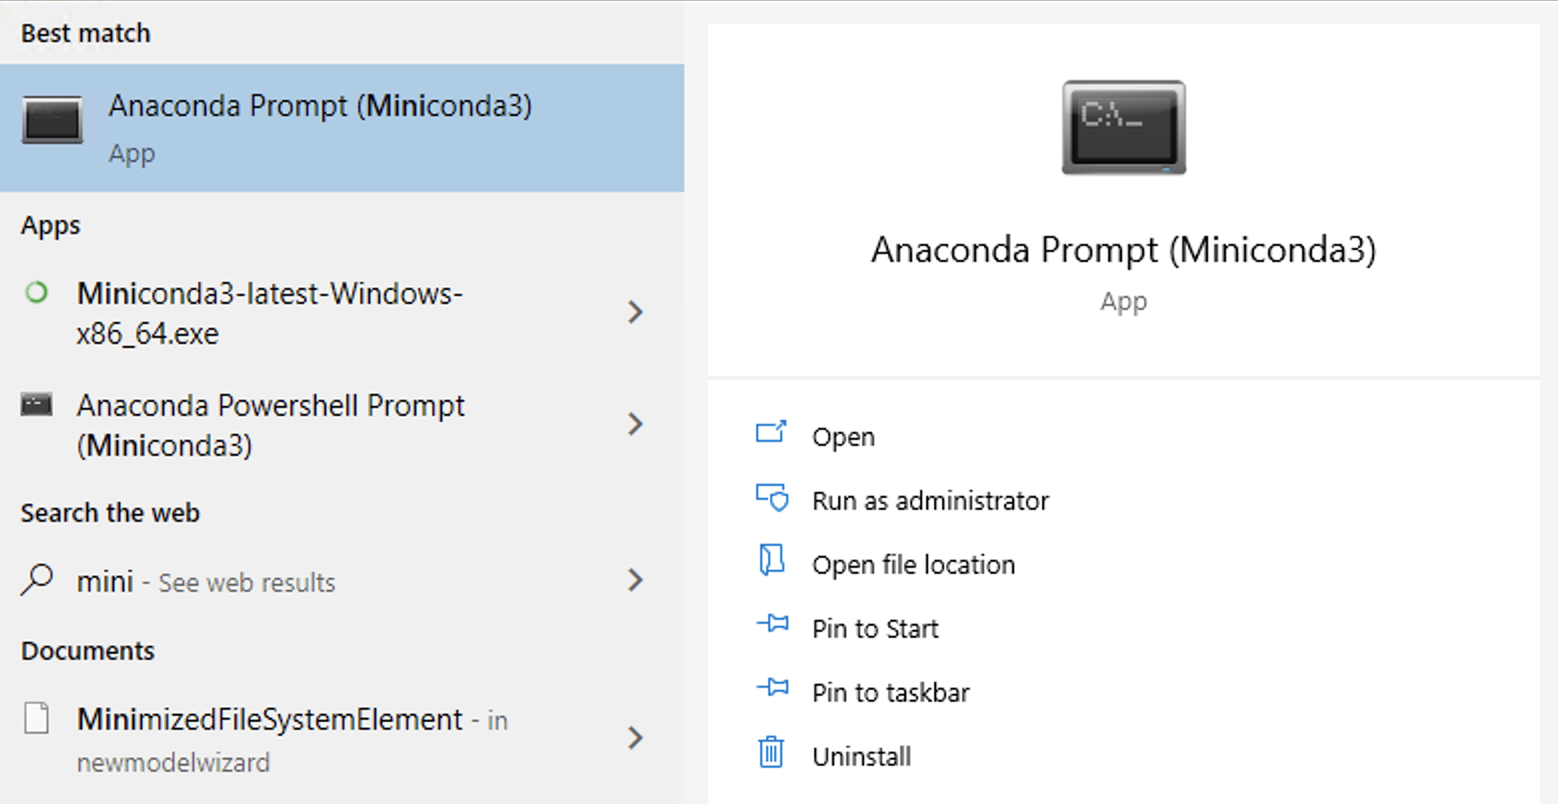
\includegraphics[scale=0.5]{acp.png} 
\end{center}


To verify the Conda download, please run: 
\begin{lstlisting}[language=bash] 
conda info
\end{lstlisting}
In case you have previously installed Conda or Anaconda, be sure to update them accordingly before moving onto step 2:
\begin{lstlisting}[language=bash] 
#Update to lastest version of Conda
conda update -n base conda
#Update all packages to the latest version of Anaconda
conda update anaconda
\end{lstlisting}

\section{Creating and activating environment from YAML file}

After you have installed Conda, we have provided a file called \textbf{environment.yml}. This YAML file will help you create a virtual environment with a specified name used for activation and install necessary dependencies for the coding assignments. Here is what an example environment.yml file looks like.
\begin{center}
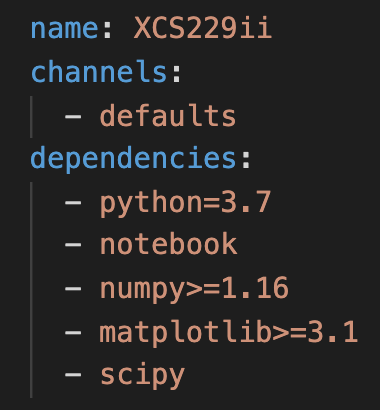
\includegraphics[scale=0.75]{conda-update.png}
\end{center}
\textbf{Note: }Although there are multiple ways of completing the homework assignments, the libraries we provide you within the YAML file should be the only ones you reference in the completion of the coding assignments. 
\textbf{For the remainder of this setup we will be using \textit{your-env-name} to specify the name of your environment (i.e. XCS229, XCS229ii, XCS221, etc) . You can find the name of your virutal environment by looking for the name parameter within the environment.yml file.} 

To create your environment from the YAML file please run: 
\begin{lstlisting}[language=bash]
conda env create --file environment.yml
\end{lstlisting}
Now to specify that the environment was installed correctly, please run the code below and you should see an environment name that matches with the name parameter in the environment.yml file:
\begin{lstlisting}[language=bash]
conda env list
\end{lstlisting}

Next, you will activate the created environment. To do so, you will need to to call the following command:
\begin{lstlisting}[language=bash]
conda activate <your-env-name>
\end{lstlisting}

Now in this environment, you will have all the relevant dependencies needed to complete the assignments. If you want to deactivate your environment please run:
\begin{lstlisting}[language=bash]
conda deactivate
\end{lstlisting}
 
\section{Converting Environment to Jupyter Notebook}
When completing the assignments, it may be helpful to use a Jupyter Notebook as a scratchpad to help you debug or formulate potential solutions. Jupyter Notebook is an open-source web application that allows you to create and share documents that contain live code, equations, visualizations and narrative text. The first step to creating your Jupyter Notebook for the assignments is to activate your environment as follows:
\begin{lstlisting}[language=bash]
conda activate <your-env-name>
\end{lstlisting}

Next, in the active environment type:
\begin{lstlisting}[language=bash]
#install ipykernel
conda install -c anaconda ipykernel
#install the new kernel
ipython kernel install --user --name=<your-env-name>
\end{lstlisting}

And last but not least, ensure to run the following command to launch your Jupyter Notebook in the active environment
\begin{lstlisting}[language=bash]
jupyter notebook
\end{lstlisting}

That command will take you to your Jupyter Notebook directory. When you hover over the \textbf{New} button in the top right hand corner, you should see you environment present as an option.
\begin{center}
   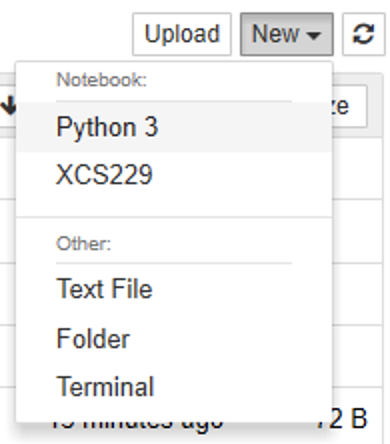
\includegraphics[]{p2.png} 
\end{center}
Go ahead and select it and it will create an empty Python Jupyter file where you can copy and paste assignment code or use it to formulate your thoughts. 

In the event you would like to remove your environment from Jupyter, simply run the following code:
\begin{lstlisting}[language=bash]
jupyter kernelspec uninstall <your-env-name>
\end{lstlisting}

You are now equipped with all the tools to complete the coding assignments. For a list of the most useful Conda functions, \href{https://docs.conda.io/projects/conda/en/latest/_downloads/843d9e0198f2a193a3484886fa28163c/conda-cheatsheet.pdf}{please refer to this document}. 

\section{Updating Existing Conda Environment}
 If you plan on reutilizing the an existing Conda environment from a previous SCPD-AI course, we strongly recommend all students update their Conda environment upon starting or replace it with the new Conda environment as mentioned above. Below are steps to update your existing Conda environment in preparation for this course. 

\begin{lstlisting}[language=bash]
conda activate <your-env-name>
conda env update --file environment.yml 
\end{lstlisting}
 
\end{document}
